% Anonymous build of the paper (no author name/email, no acknowledgments).
% Shares body/tables/refs with paper.tex. Build from this directory:
%   lualatex paper_anonymous.tex && bibtex paper_anonymous && lualatex paper_anonymous.tex && lualatex paper_anonymous.tex
% Output: paper_anonymous.pdf
\def\AnonymousVersion{}
\documentclass[11pt]{article}
\usepackage[margin=1in]{geometry}
\usepackage{booktabs}
\usepackage{multirow}
\usepackage{graphicx}
\usepackage{amsmath}
\usepackage{amssymb}
\usepackage[numbers,sort&compress]{natbib}
\setlength{\bibsep}{2pt plus 1pt}
\usepackage{caption}
\usepackage{newtxtext}
\usepackage[dvipsnames]{xcolor}
\usepackage{hyperref}
\usepackage{eso-pic}
\captionsetup{font=small,labelfont=bf}
\captionsetup[table]{font=small,labelfont=bf}
\hypersetup{
  colorlinks=true,linkcolor=black,citecolor=NavyBlue,urlcolor=NavyBlue,
  pdfauthor={},
  pdftitle={The Vector Is the Answer? One-Pass Residual Readouts vs Fair Loop Scoring},
}
\newcommand{\drafttimestamp}{%
  \number\day/\number\month/\number\year\space
  \directlua{tex.sprint(os.date("!"..string.char(37).."H:"..string.char(37).."M"))}%
}

% ArXiv-style draft marker in the outer margin; this is an overlay and does not
% affect the paper's layout or pagination.
\AddToShipoutPictureFG{%
  \AtPageLowerLeft{%
    \put(22,0){\color{gray!35}\rule{1pt}{\paperheight}}%
    \put(25,365){%
      \rotatebox{90}{%
        \sffamily\bfseries\fontsize{8}{8}\selectfont\color{gray!65}%
        DRAFT\ --\ \drafttimestamp}%
    }%
  }%
}

\newcommand{\sd}[1]{\textbf{#1}}
\newcommand{\pstar}{$^{*}$}
\newcommand{\pstarstar}{$^{**}$}
\newcommand{\pstarstarstar}{$^{***}$}
\newcommand{\head}{readout}
\newcommand{\loopk}{loop.$k$}

\title{\textbf{The Vector Is the Answer?\\
One-Pass Residual Readouts vs Fair Loop Scoring}}
\ifdefined\AnonymousVersion
\author{Anonymous Author(s)}
\date{}
\else
\author{
  Hanan Herzog\\
  \texttt{hanan.herzog@gmail.com}
}
\date{}
\fi

\begin{document}
\maketitle

\begin{abstract}
Language models usually answer classification questions by generating an answer
token, but their internal representation may already contain the information
needed to choose the correct answer. We test this by comparing two ways of
answering questions with a fixed choice set. The first is a small classifier
on the frozen residual after one forward pass. The second is fair closed-set
scoring: the model sees the question and balanced few-shot examples, and we
compare answer-token probabilities rather than free-form or multi-step
generation. The classifier is trained on the gold training split; the loop
is few-shot scoring, not a fine-tuned decoder.

We evaluate on BoolQ, RuleTaker, and ARC-Challenge with six open-weight models
from 0.6B to a mixture-of-experts model. The one-pass classifier matches or
beats token scoring on BoolQ and RuleTaker except two cells (Mistral-7B on
BoolQ; DeepSeek-V4-Flash on RuleTaker). On ARC-Challenge the scorer wins when
the one-pass classifier is still weak --- that tracks probe accuracy, not
model size --- including an 8.2-point gap on Granite-3.1-8B. The
classifier's largest gain is 11.9 points on RuleTaker with Granite-3.1-8B,
where token probabilities are weakest. Label-shuffle, random-projection, and
paired tests support the comparison. Sweeping the tap across depth, the best
mid-layer readout beats the final layer in 10 of 18 cells after correction and
never loses significantly. That is what a small readout can extract, not a
license to skip later layers. For this task class the vector often already
contains the answer; the loop still wins on ARC when the probe is weak.
\end{abstract}

\section{Introduction}

Autoregressive decoding is the usual interface to a language model, but it is
only one readout of a residual vector that already exists after a single
forward pass. On closed-set classification, does that vector already contain
the gold label?

We compare two readouts of the same frozen model. The \emph{one-pass
\head{}} is a small classifier --- logistic regression or a one-hidden-layer
MLP --- fit to the final-token residual after one prompt pass; the backbone
is never updated. Linear probes sit within a few points of the MLP
(\S\ref{sec:boolq}). The \emph{fair loop} is closed-set scoring: the model
sees the question plus balanced few-shot exemplars, and we compare next-token
log-probabilities over the answer set. Zero-shot prompting understates this
baseline \citep{cho2025hidden}. A probe that recovers the model's self-report
shows beliefs are present, not that a \head{} matches a fair loop at the gold
label.

The loop is given balanced few-shot exemplars and a longer context than the
\head{} (deliberately; \S\ref{sec:setup}). The \head{} is fit on the training
split. Extra in-context shots do not erase the pattern on BoolQ
(\S\ref{sec:boolq}). We report label-shuffle nulls, random-projection
selectivity, and paired tests.

\textbf{Concurrent work.} \citet{hazenoot2026esg} find a linear probe on frozen
activations beats the same model's prompted yes/no on ESG concept measurement
(11/12 comparisons), mid-network. Their baseline is zero-shot prompting, which
understates the loop (\S\ref{sec:boolq}), and they report no paired
significance or selectivity controls.

\textbf{Findings.} BoolQ (full validation, 3270 rows), RuleTaker (10k/4k),
ARC-Challenge (full test); six models from 0.6B to a frontier MoE:

\begin{enumerate}
\item \textbf{BoolQ and RuleTaker: match or win, with two exceptions.} The
  one-pass \head{} matches or beats the fair scorer except Mistral-7B on BoolQ
  ($-2.2$pt) and DeepSeek-V4 on RuleTaker ($-1.6$pt). Four of six BoolQ cells
  are statistical ties within $\pm$1.2pt (\S\ref{sec:boolq}, \S\ref{sec:tasks}).
\item \textbf{On ARC the loop wins when the probe is weak.} The
  gap tracks probe accuracy, not parameter count: Qwen $-10.6 \to -4.1 \to
  -0.4$pt (the last ns); Granite-8B still loses by $8.2$pt at readout
  accuracy 0.708 (\S\ref{sec:boundary}).
\item \textbf{Answer-relevant information is already present mid-depth.} The
  best mid-layer tap beats the final layer at 11/18 cells (10/18 after
  Benjamini--Hochberg) and never loses. That is what a small readout can
  extract from $h_l$, not a claim that later layers can be skipped
  (\S\ref{sec:placement}).
\item \textbf{The margins can be large.} Where token probabilities are
  weakest, the \head{}'s lead is largest: $+11.9$pt on RuleTaker with
  Granite-3.1-8B (\head{} 0.823 vs loop 0.703, McNemar $p=1.1\mathrm{e}{-45}$).
\end{enumerate}

Fine-tuned specialist encoders beat our \head{}; serial-depth tasks may
require the loop; a frozen latent loop drifts
(\S\ref{sec:boundary}, \S\ref{sec:discussion}). The result is for this task
class, not early exit and not all tasks.

\textbf{Scope.} A companion position paper explores a serving architecture of
kilobyte-scale \head{} heads (Paper~2). This paper contains no architecture
claims and no production system.

\section{Setup and Method}
\label{sec:setup}

\subsection{Two readouts of the same vector}

\textbf{One-pass \head{}.} Let $h_T \in \mathbb{R}^d$ be the final-token
residual of a frozen model after one forward pass over the task prompt
(question $+$ passage, truncated at $\mathrm{pad\_max}=384$). We fit a head
$f(h_T) \to \hat{y}$: either multinomial logistic regression or a
one-hidden-layer MLP (width 128, 4-seed vote), both on standardized features.
The head sees only task labels; the backbone is never updated.

\textbf{Fair loop.} The autoregressive baseline is \emph{not} greedy decode
--- it is the strongest \emph{classifier} the loop provides. The model receives the
full context (balanced few-shot exemplars, $\mathrm{loop\_pad\_max}$
2048--8192) and is scored by next-token log-probability over the closed answer
set (Yes/No, or A--D). We report loop.0 (zero-shot) and loop.$k$ ($k$-shot);
where noted we sweep $k$ up to 64 with a $4\times$ pad budget.
\emph{Scope:} we evaluate the strongest \emph{classifier} the loop offers, not
a chain-of-thought loop that generates intermediate tokens before answering.
Generated-then-answered chains are a different readout, break the matched
closed-set scoring protocol, and --- on a serial task such as RuleTaker ---
require intermediate generation by construction; they are out of scope for the
matched comparison.

\subsection{Matching requirements}

A \head{}-vs-loop comparison is only meaningful if the loop is not
handicapped. We match \textbf{scoring} (same closed answer set, accuracy on
identical rows). On \textbf{information} we advantage the loop: both see the
same question and passage, and the loop also sees $k$ balanced exemplars from
the training split plus a longer pad ($2048$--$8192$ vs.\ the \head{}'s
$384$). That is conservative for the \head{}: the loop sees more of the
passage and the exemplars. The \head{} is a probe fit on the training labels;
the loop is in-context scoring. We sweep the loop to $k{\le}64$ at
$4\times$ pad on BoolQ at 0.6B/4B/8B; extra shots plateau and do not pass the
\head{} where it was winning (\S\ref{sec:boolq}).

\subsection{Controls}

Every headline number carries four controls:

\begin{itemize}
\item \textbf{Label-shuffle null}: the head refit on
  permuted labels must sit at chance, ruling out leakage and spurious
  separability.
\item \textbf{Random-projection selectivity}: a head on
  random Gaussian projections of the residual. If it retains accuracy, the
  signal is \emph{diffuse} --- no privileged subspace --- which is what we
  find (permuted-basis $\approx$ max-basis $\gg$ noise floor) at every scale.
\item \textbf{Final-token vs full-context}: a mean-pooled
  full-context \head{} must underperform the final-token \head{}, confirming
  the verdict is \emph{computed into} the final state rather than read off the
  passage surface.
\item \textbf{Paired significance}: McNemar's exact test and paired bootstrap
  on per-row predictions from identical val rows,
  not pooled-accuracy eyeballing.
\end{itemize}

On BoolQ at DeepSeek-V4 we also re-score within question- and passage-length
terciles (accuracy 0.89--0.90, flat). That is a coarse check that the
\head{}'s edge is not an artifact of the loop truncating long rows; it is
not a control on every cell.

\subsection{Models and artifacts}

Six open-weight models spanning three families and a width ladder: Qwen3-0.6B
($28{\times}1024$), Qwen3-4B ($36{\times}2560$), Qwen3-8B ($36{\times}4096$),
Mistral-7B ($32{\times}4096$), Granite-3.1-8B ($40{\times}4096$),
DeepSeek-V4-Flash ($43{\times}4096$, FP8 MoE). All runs are batch 8 on
model-pinned GPUs (0.6B/4B H200, 8B/Mistral/Granite B200, DSV4 B300). Trained
heads are persisted per layer as versioned artifacts ($\sim$0.5--8.4\,MB each);
per-row predictions persist for paired tests. Run manifests embed the batch
tag in cache keys.

\section{BoolQ: one-pass \head{} vs the fair loop}
\label{sec:boolq}

BoolQ \citep{clark2019boolq} is binary reading comprehension with the gold
answer grounded in a passage --- the cleanest closed-set case in which to test
whether one prompt forward pass already carries the label. We load the standard Hugging Face release (\texttt{google/boolq}) and
use the full validation split (9427 train / 3270 val).

\subsection{Headline}

Across the Qwen and Granite scales, the one-pass \head{} \textbf{wins at
0.6B, is a statistical tie at 4B/8B (numerical losses ${\sim}$0.8--1.2pt,
ns), and trails the few-shot loop by $\sim$1pt (ns) at Granite-8B and the
frontier MoE} (Table~\ref{tab:main}). The one exception is Mistral-7B, where
the loop wins by $2.2$pt ($p=2.6\mathrm{e}{-03}$) --- the single significant
loop win on BoolQ, which we flag as a single-model exception
(\S\ref{sec:discussion}).

\begin{figure}[t]
\centering

\includegraphics[width=\columnwidth]{figures/boolq_results.png}
\caption{\textbf{BoolQ: \head{} vs loop} across six models (full val).}
\label{fig:boolq}
\end{figure}

\subsection{Extra in-context shots do not close the gap}

The natural objection: the head sees thousands of labels, the loop sees $k$
exemplars. We gave the loop its budget back --- $k$ swept to 64 balanced
exemplars at $4\times$ pad (8192) --- at 0.6B/4B/8B. The loop's $k$-curve
\textbf{plateaus by $k{=}32$} (loop.64 $-$ loop.32 $=-0.0003$, $p=1.00$ at
0.6B) and \textbf{never passes the \head{} where the \head{} was winning}: at
0.6B the \head{}'s $+3.0$pt over the best loop stays significant
($p=3.2\mathrm{e}{-05}$); at 4B/8B all cells are exact ties. More in-context
supervision does not explain the 0.6B win (Fig.~\ref{fig:kcurve}).

\begin{figure}[t]
\centering

\includegraphics[width=\columnwidth]{figures/boolq_budget_kcurve.png}
  \caption{\textbf{Supervision budget.} The loop's $k$-curve plateaus
by $k{=}32$ and never passes the \head{} on BoolQ.}
\label{fig:kcurve}
\end{figure}

\subsection{Readings}

\begin{enumerate}
\item \textbf{Parity or better at five of six models; the edge is largest
  where the model is weakest.} The \head{}'s only significant win is at 0.6B
  --- the loop's verbal channel is the bottleneck there, and the \head{}
  channel saturates before it. Mistral-7B is the exception (loop $+2.2$pt).
\item \textbf{The signal is distributed, not localized.} Random-projection
  heads retain accuracy (perm $\approx$ max $\gg$ noise) at every scale; no
  privileged subspace carries the verdict (Table~\ref{tab:controls}).
\item \textbf{The verdict concentrates in the final token.} Mean-pooled
  full-context \head{}s underperform the final-token \head{} everywhere
  (full-context $\ll$ final-token) --- the answer is computed into the final
  state, not read off the passage.
\item \textbf{The readout is essentially linear.} A multinomial logistic
  \head{} tracks the MLP within a few points at every scale (BoolQ 0.6B
  linear.max 0.750 vs MLP 0.747; 8B 0.874 vs 0.881), so the verdict is a
  near-\emph{linear} read of the residual, not a fragile nonlinear probe. At
  0.6B, where the residual does not yet hold the answer (ARC $\approx$0.49,
  near chance), no head can invent it --- the \head{} reads what is there.
\end{enumerate}

\emph{Context length.} The \head{} reads at $\mathrm{pad\_max}=384$ against
the loop's 2048--8192. Because the BoolQ gold answer is grounded in the
passage, left-truncation could in principle drop long passages
asymmetrically; we do not log per-row truncation rates and flag this as a
limitation (\S\ref{sec:limits}), noting the length-tercile check in
\S\ref{sec:setup} shows no length-dependent accuracy collapse.

\subsection{Scoring vs decoding}

Readout and scoring loop are both one context forward pass, unequal only in
context length. A decode loop is a different, more expensive readout. In a
small check, greedy decode from an ``Answer:'' prompt hit the length cap
(25/25 at 300 tokens on 0.6B; 7/8 at 1000 tokens on DeepSeek-V4). That is
not a latency benchmark.

\section{RuleTaker and ARC: serial depth and parametric knowledge}
\label{sec:tasks}

BoolQ is passage-grounded. We test the two ways a task can be harder for a
one-pass \head{}: \textbf{serial deduction depth} (RuleTaker) and
\textbf{parametric knowledge with no passage} (ARC-Challenge).

\subsection{RuleTaker 10k/4k: matched loop rows, per-depth strata}

RuleTaker \citep{clark2020ruletaker} is closed-world rule reasoning with
labeled deduction depth (0/1/2/3/5 $+$ NatLang), loaded via Hugging Face
\texttt{tasksource/ruletaker}. Protocol: 10000 train / 4000 val (subsample of
the full release), loop on the same 4000 rows, $k\in\{0,8\}$,
batch 8. On Qwen, the matched one-pass MLP \textbf{beats
the fair loop at every scale} ($+4.6$ to $+9.2$pt; all $p{<}10^{-8}$; 0.6B
prefers zero-shot, 4B/8B prefer 8-shot). The cross-family models sharpen the picture:
Mistral-7B $+11.1$pt ($p=4.2\mathrm{e}{-28}$), \textbf{Granite-3.1-8B $+11.9$pt
($p=1.1\mathrm{e}{-45}$) --- the largest \head{} margin we measure.} The
one clean loop win is DeepSeek-V4 ($-1.6$pt,
$p=0.029$), driven by the shallow-depth strata.

\textbf{Per-depth} (same rows): no sharp ``only the loop works past depth
$D$'' cliff. Accuracy degrades gradually with depth; $d{=}5$ remains well
above chance. The DSV4 loop win concentrates at shallow depths ($d0/d1$,
$+5$--$11$pt); at 0.6B the loop lags at depth ($d5$ loop.8
0.522 vs.\ \head{} 0.625). Depth bins are $n{=}211$--$1946$ ($d3$ dominates)
(Fig.~\ref{fig:depth}).

\begin{figure}[t]
\centering
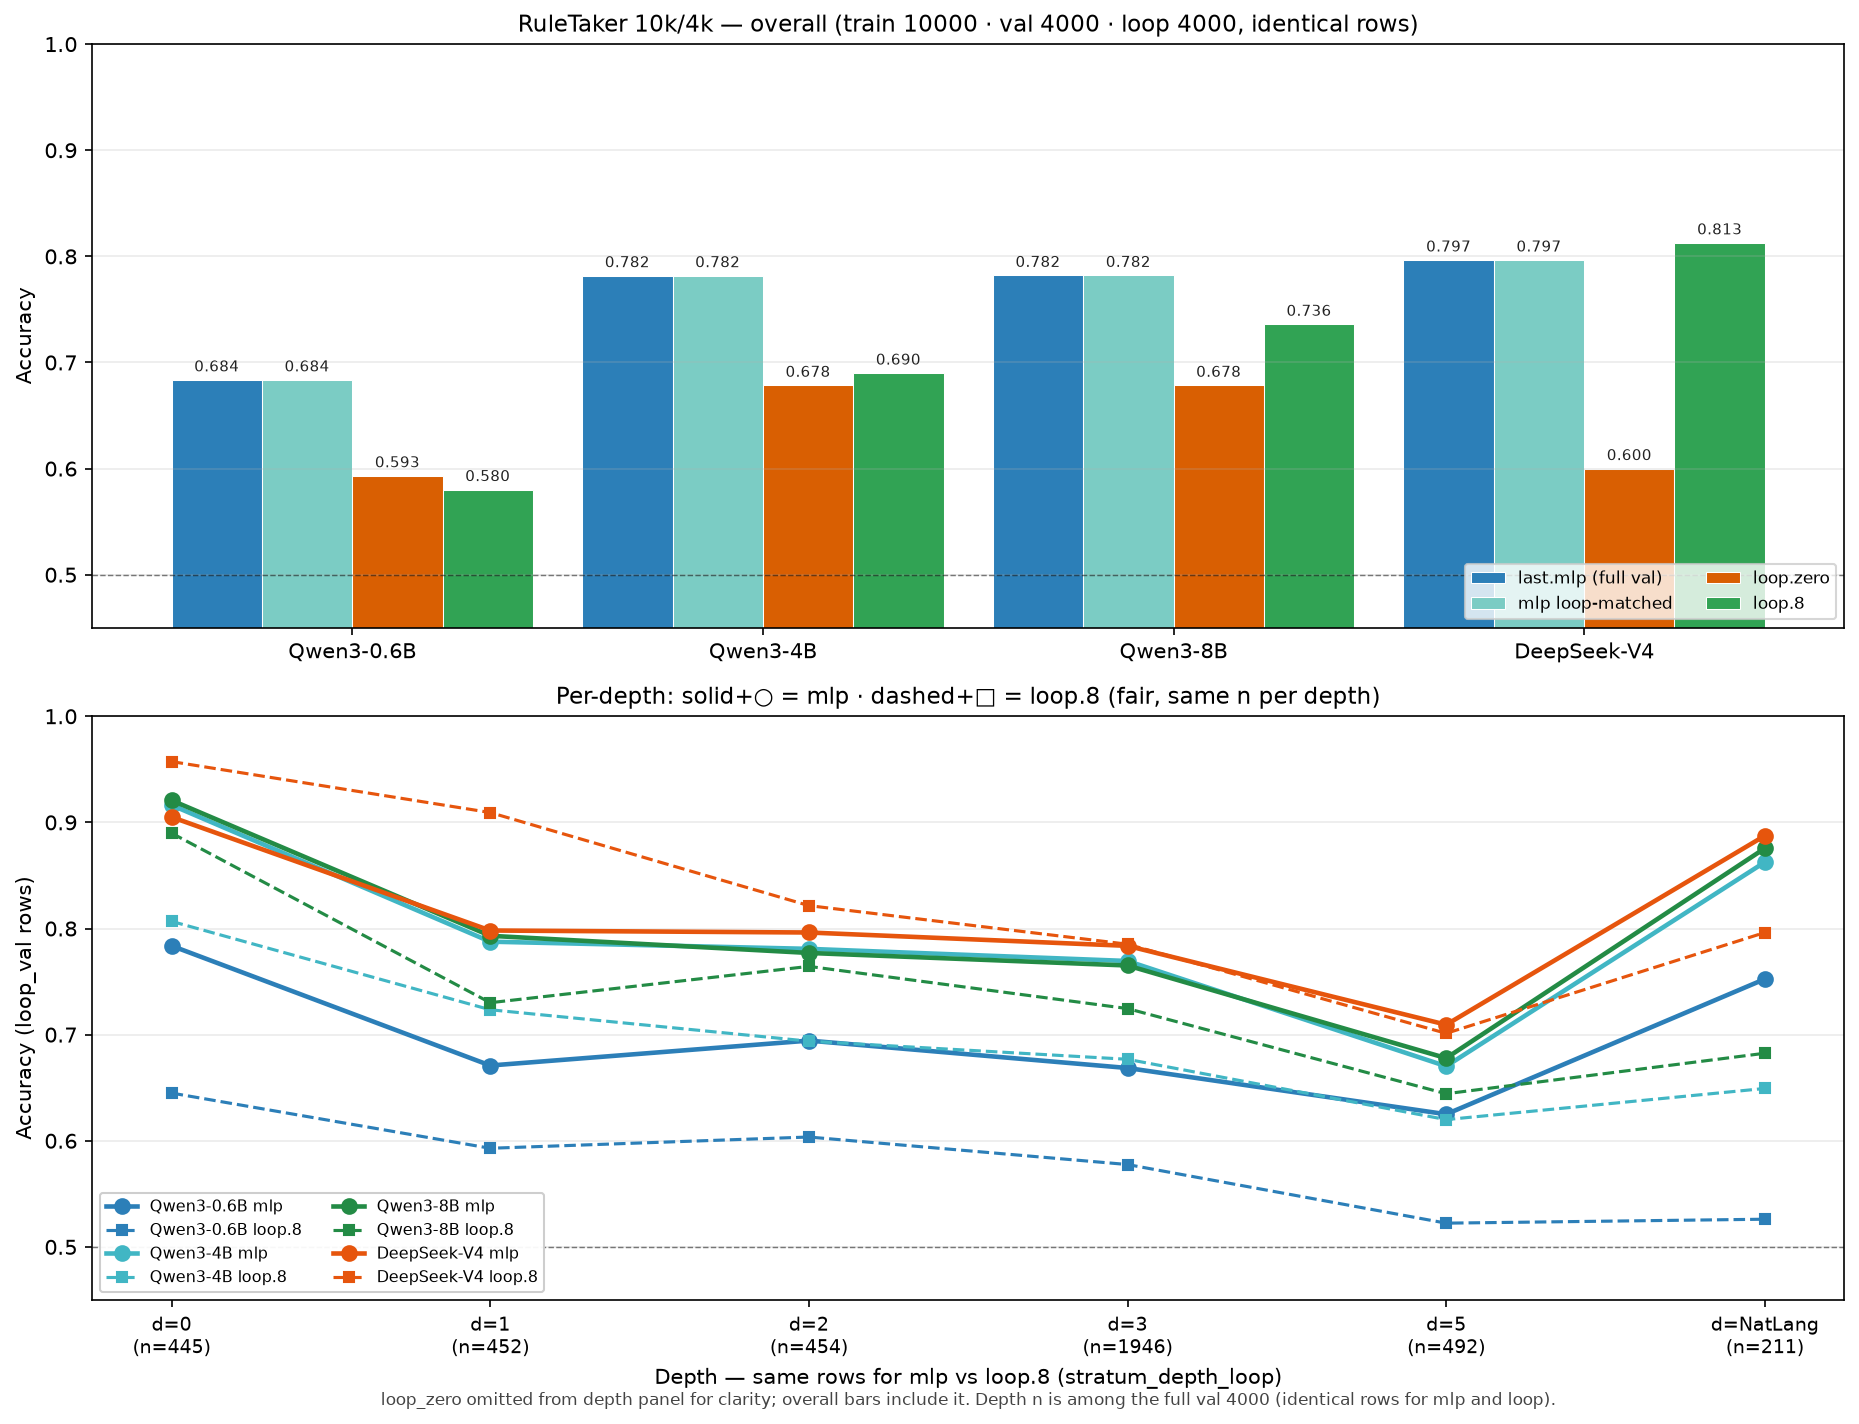
\includegraphics[width=\columnwidth]{figures/ruletaker_depth_strata.png}
\caption{\textbf{RuleTaker overall $+$ per-depth strata}, \head{} vs loop.}
\label{fig:depth}
\end{figure}

\subsection{ARC-Challenge: the loop's best case}

ARC-Challenge \citep{clark2018arc} is the hard partition of the AI2 Reasoning
Challenge (not Chollet's Abstraction \& Reasoning Corpus): grade-school science
multiple-choice questions that retrieval and co-occurrence baselines miss. We
load \texttt{allenai/ai2\_arc} config \texttt{ARC-Challenge} and keep 4-choice
A--D items only ($\sim$99\% of the set). Answers are parametric science
knowledge with no passage --- they must come from the weights, not the
context. On Qwen the loop beats the one-pass classifier at 0.6B ($-10.6$pt)
and 4B ($-4.1$pt; both $p<1\mathrm{e}{-05}$). At 8B and DeepSeek-V4 the
gap is gone ($-0.4$pt and $-1.0$pt, both ns). Cross-family
models sit with Qwen at matched readout accuracy, not matched size:
Mistral-7B $-5.1$pt ($p=9.3\mathrm{e}{-05}$), Granite-8B $-8.2$pt
($p=5.8\mathrm{e}{-10}$). Few-shot exemplars teach a task format the residual
head must otherwise learn from labels; the gap shrinks as probe accuracy
rises.

\subsection{The task-type regularity}

Across 18 task$\times$model cells the organizing fact is capability on ARC,
not three special regimes (Fig.~\ref{fig:tasklaw}). \textbf{The loop wins
on ARC when the one-pass classifier is still weak} (Qwen 0.6B/4B, Mistral,
Granite). Elsewhere the one-pass \head{}
wins or ties, with two exceptions: DeepSeek-V4 on RuleTaker and Mistral-7B
on BoolQ. Granite/Mistral sit where Qwen did at equal ARC accuracy, not
equal size. The Mistral BoolQ cell is a single-model exception we flag
rather than explain (\S\ref{sec:discussion}).

\begin{figure*}[t]
\centering
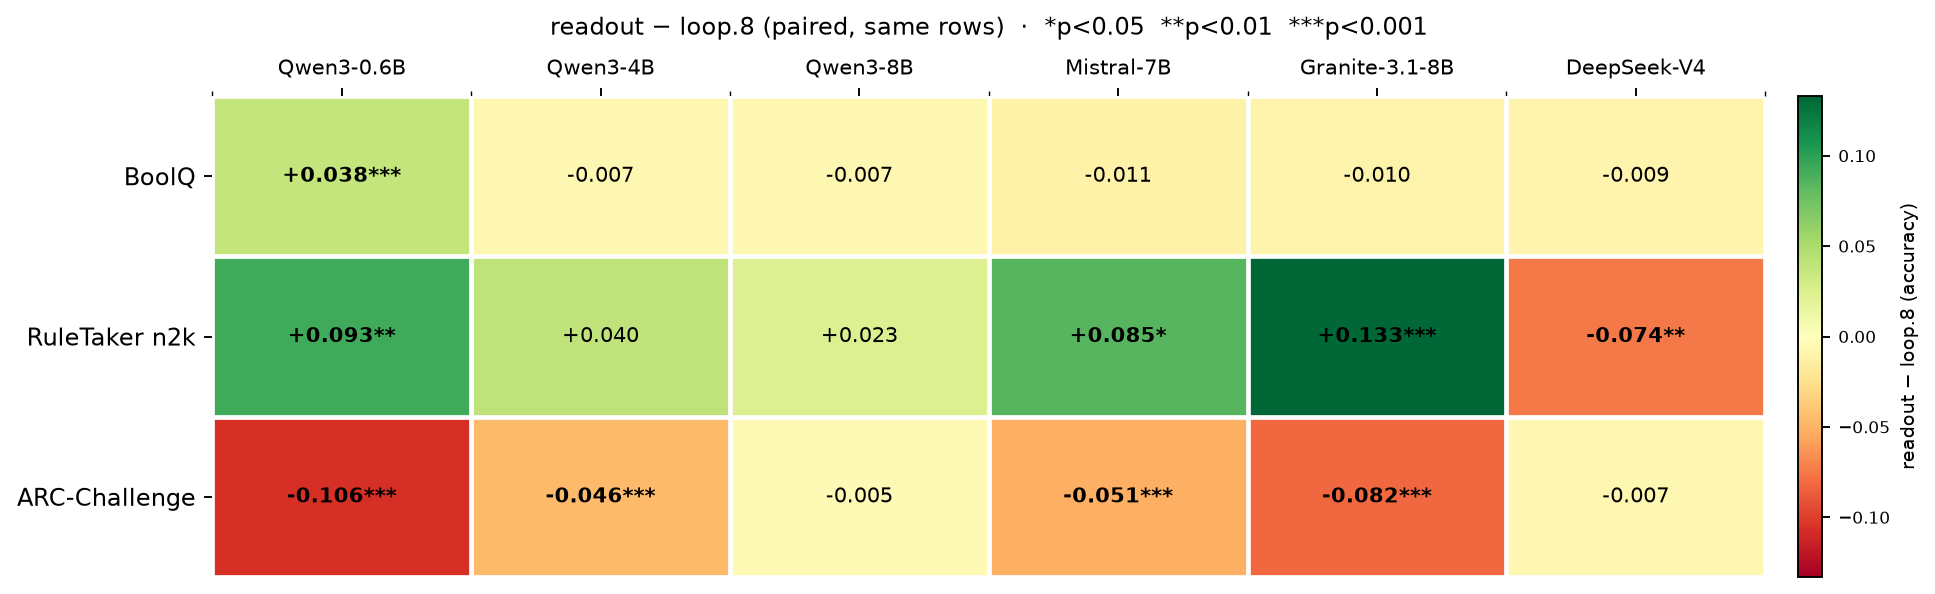
\includegraphics[width=\textwidth]{figures/tasklaw_summary.png}
\caption{\textbf{Readout $-$ best loop} (paired, same rows) per
task$\times$model cell, with McNemar significance. The loop's significant
wins cluster on ARC at low probe accuracy, plus DeepSeek-V4
RuleTaker and Mistral-7B BoolQ.}
\label{fig:tasklaw}
\end{figure*}

\begin{figure}[t]
\centering

\includegraphics[width=\columnwidth]{figures/head_to_head_three_tasks.png}
\caption{\textbf{Three-task head-to-head} (BoolQ $\cdot$ RuleTaker $\cdot$
ARC) across models.}
\label{fig:h2h}
\end{figure}

\subsection{Readout placement: information across depth}
\label{sec:placement}

Every headline number above taps the final residual layer. We swept the tap
across depth (10 layers, paired McNemar vs the final-layer \head{}, trained
heads persisted at every tap). The curve is the same everywhere: monotone
rise, mid-depth plateau, slight terminal decline (Table~\ref{tab:placement},
Fig.~\ref{fig:placement}). A high mid-depth readout accuracy means the residual
already contains extractable answer-relevant information; it does not mean
the intermediate LM head is correct, or that stopping there reproduces
full-model behavior.

\begin{itemize}
\item \textbf{The final-layer readout is not the best readout.} Mid-depth taps
  beat the final layer significantly at \textbf{11/18 cells and never lose
  significantly} --- the headline numbers were a lower bound on what a
  gold-label \head{} can extract, not a claim that later layers add nothing.
  Across the 18 cells, 10 survive a Benjamini--Hochberg FDR correction at
  $q<0.05$ (only BoolQ 4B drops); the ``never loses'' direction is unchanged.
\item \textbf{The optimum is task-stable, not scale-driven.} BoolQ/RuleTaker
  peak at 50--86\% depth at every scale; RuleTaker's Qwen and DeepSeek-V4
  optima sit at $\sim$2/3 depth, while Mistral peaks at mid-stack (L16/32).
  ARC drifts to the final layer at $\ge$8B ---
  once the parametric answer saturates the residual, late-layer specialization
  stops costing anything.
\item \textbf{A mid-layer tap can beat the final-layer tap.} Where the loop
  catches the final-layer \head{} (BoolQ 8B: L35 ties the loop), the best
  mid-layer tap beats the final layer (L30 $+1.1$pt vs L35, $p=0.016$;
  Granite L20 $+1.4$pt vs final, $p=1\mathrm{e}{-03}$). That is not
  automatically a win against the loop (BoolQ 8B L30 0.889 vs best loop
  0.886).
\item \textbf{Wide-shallow plateaus earlier.} Mistral ($32{\times}4096$)
  onsets at 35--58\% depth vs Qwen3-8B's uniform 69\% at the same width --- at
  fixed width, the shallower stack yields a usable label signal sooner. Granite
  ($40{\times}4096$, deep) sits between the two.
\end{itemize}

\begin{figure*}[t]
\centering

\includegraphics[width=\textwidth]{figures/layersweep_placement.png}
\caption{\textbf{Readout probe-placement sweeps} (18 cells). One-pass \head{}
accuracy vs tapped residual layer; loop arms as horizontal references; paired
McNemar annotation per panel. Mid-depth taps win significantly at 11/18 cells
and never lose.}
\label{fig:placement}
\end{figure*}

\emph{Causal hedge.} The monotone-rise $\to$ plateau $\to$ terminal-decline
shape is \emph{consistent with} late-layer specialization toward next-token
surface form or confidence correction, but we do not demonstrate it: we never
ablated deep layers against generation, never measured calibration vs.\
correctness by layer, and never probed next-token structure per layer. Three
claims should not be conflated: (i)~the intermediate LM head predicts the
correct token; (ii)~a small readout can extract the gold answer from $h_l$;
(iii)~stopping at layer $l$ reproduces full-model behavior. The placement
sweep addresses (ii). Inferring (iii) from (ii) is the early-exit claim, and
it is prior art we do not make (\S\ref{sec:related}).

\section{The boundary: where the loop could win, and why it doesn't cleanly here}
\label{sec:boundary}

A single forward pass is a bounded-depth computation (TC$^0$ in the circuit-
complexity framing); the loop's advantage should appear exactly where serial
depth is irreducible. We hunted that regime and found it only weakly
exhibitable on frozen base weights:

\begin{itemize}
\item \textbf{RuleTaker per-depth} shows a gentle slope, not a regime switch
  --- the loop edges the \head{} by a few points at $d{=}5$ (noisy thin bins),
  and the one decisive loop win (DSV4) concentrates at \emph{shallow} depths,
  where the frontier model's in-context deduction is strong.
\item \textbf{ARC} shows the loop's real advantage is \emph{parametric
  retrieval under a learned task format}, not serial compute --- and it closes
  with scale.
\item \textbf{Synthetic mechanism} (multi-hop transitivity with shuffled
  facts; Fig.~\ref{fig:synthetic}): the relation is linearly decodable from
  the frozen residual (0.93--0.97) where the zero-shot decoder sits at chance;
  a 2-demo budget surfaces the loop's inference but never exceeds the one-pass
  MLP. The measured limit is \textbf{order-locked binding}, not depth.
\end{itemize}

\begin{figure}[t]
\centering
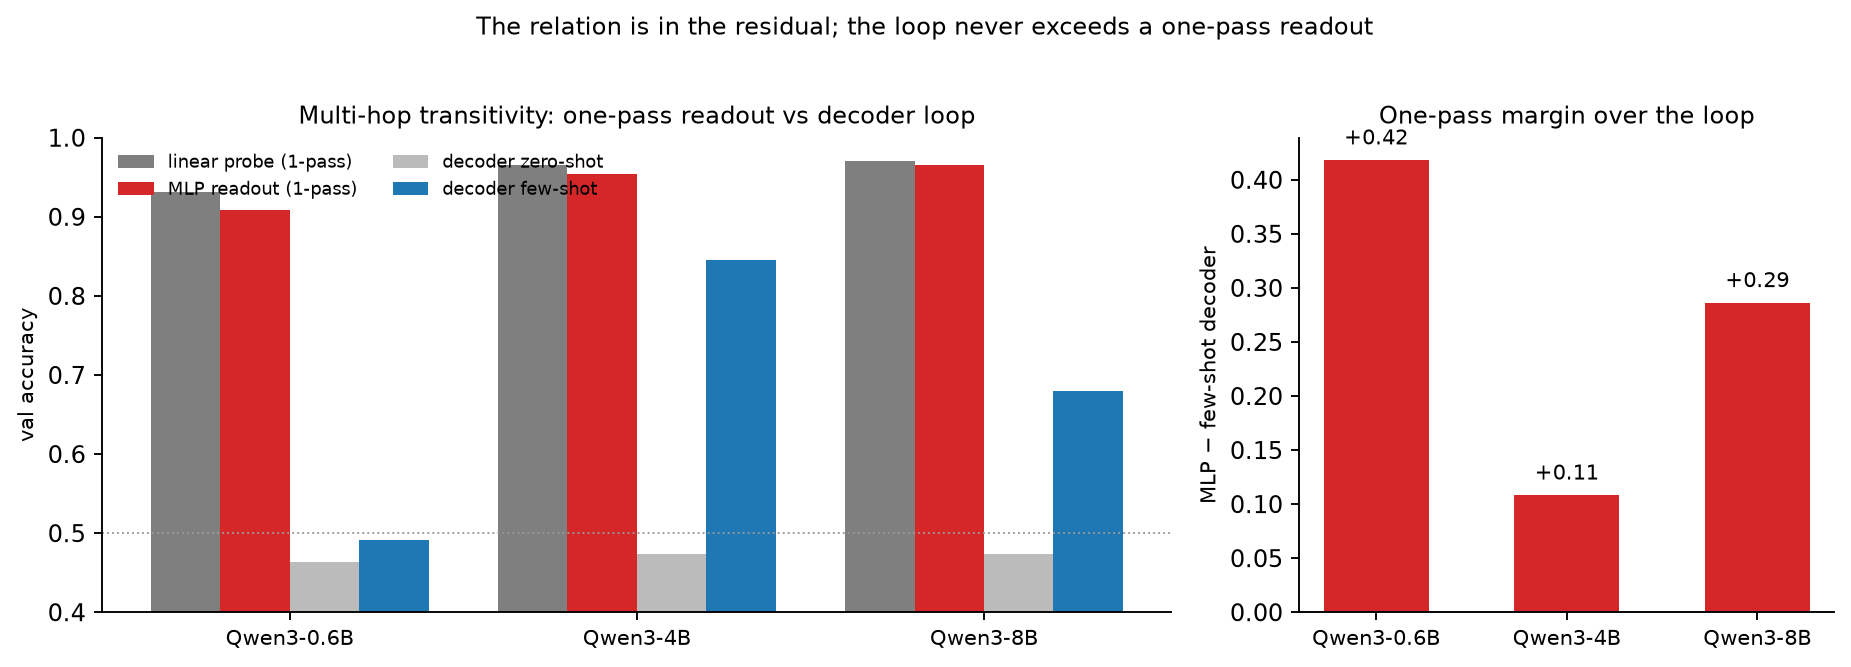
\includegraphics[width=\columnwidth]{figures/synthetic_multihop.png}
\caption{\textbf{Mechanism (synthetic).} Multi-hop transitivity: one-pass
\head{} vs decoder loop across Qwen3 scale. The loop never exceeds a one-pass
\head{}.}
\label{fig:synthetic}
\end{figure}

The remaining ``loop wins'' cell --- a TC$^0$-hard task on which a
\emph{frozen} loop decisively beats one-pass --- is largely unoccupied in our
sweep; the counter-position (COCONUT, looped-latent) buys serial depth by
\emph{training}, which is out of scope here. Because RuleTaker is a 10k/4k
subsample of the official release ($d3$ fat), we treat the serial-depth
boundary as \emph{indicative}: it shows where a TC$^0$ gap would appear
but does not pin its location on the full test.

\section{Discussion}
\label{sec:discussion}

On closed-set classification with a fixed answer set, a single prompt forward
pass is enough: a small head on the frozen residual matches a fair
autoregressive classifier on most of this task class, so the answer is often
already in the vector. The loop still wins on ARC when the probe is weak,
and in two other cells (\S\ref{sec:boundary}).

\textbf{The residual supports a competitive closed-set classifier.} The
\head{}'s largest margins are exactly where the loop is weakest (Granite
RuleTaker $+11.9$pt; 0.6B BoolQ and RuleTaker) --- the \head{} channel saturates
before the verbal channel. This matches the
internal-knowledge/external-behavior disconnect
\citet{orgad2025know} document and \citet{gekhman2025insideout} formalize as
\emph{hidden knowledge}: a producer \head{} on the prompt residual can match
the classifier the loop provides on this task class. The \head{} is
near-linear (\S\ref{sec:boolq}): the answer is a near-linear read of a vector
the model already computes.

\textbf{The Mistral BoolQ exception.} Mistral-7B is the one model where the
loop significantly wins on BoolQ ($-2.2$pt, $p=2.6\mathrm{e}{-03}$). It is a
single-model, single-task cell, and Mistral's wide-shallow stack
($32{\times}4096$) plateaus earliest of the six models
(\S\ref{sec:placement}), so its final-layer residual is the weakest readout
substrate relative to its own loop.

\textbf{Separability of \head{} from generative interface.} The unembedding is
one \head{} of the residual --- a fixed, next-token-trained one. That a
supervised head matches it is the default expectation once stated that way;
the empirical content is \emph{where} it fails (ARC before the residual
saturates; DeepSeek-V4 on RuleTaker)
and that the failure modes are orderly.

\textbf{Specialist frontier (acknowledged).} Fine-tuned encoder classifiers
(RoBERTa-large $\sim$0.87, DeBERTa-v3 $\sim$0.88, T5-11B 0.91 on BoolQ)
\textbf{beat} our 8B one-pass \head{} (0.878). Our claim is \head{}-vs-loop on
a frozen backbone --- the comparison a serving stack faces when the weights
are already loaded --- not \head{}-vs-fine-tuned-specialist. Where a
specialist can be trained and shipped, it wins on raw accuracy; the \head{}'s
economics are marginal-cost (the forward pass already happened).

\textbf{What we are not claiming.} A frozen continuous latent loop works (it
drifts); the loop never computes; we beat fine-tuned specialists; we
shipped residual-first inference; we introduce early exit or adaptive
computation; intermediate confidence is a stop rule; later layers can be
skipped because a mid-depth readout is accurate. Paper~2 explores the serving
architecture as a proposal.

\section{Limitations}
\label{sec:limits}

\begin{itemize}
\item \textbf{RuleTaker is a 10k/4k subsample} of the official release
  (natural depth mix, $d3$ fat), not the full test; per-depth bins are
  $n{=}211$--$1946$.
\item \textbf{Multiple testing}: Table~\ref{tab:main}'s 18 McNemar $p$-values
  are reported uncorrected (stars);\\
  all 12 raw-significant cells survive the
  Benjamini--Hochberg FDR correction at $q{<}0.05$. Placement is stricter: 1
  of 11 raw mid-depth wins drops under the same correction (10/18 remain).
\item \textbf{Truncation is not logged per row}: the \head{} reads at
  $\mathrm{pad\_max}=384$ (left-truncated) against the loop's 2048--8192, and
  we do not record the fraction of rows truncated, so a length-asymmetric
  truncation cost on long-passage rows cannot be ruled out from the logged
  data (the per-length deconfound shows no accuracy collapse, but it is a
  coarse check).
\item \textbf{Probe vs few-shot scorer}: the \head{} is fit on the training
  split; the loop is in-context scoring, not a fine-tuned decoder. On BoolQ
  the loop's $k$-curve plateaus by $k{=}32$ and never passes the \head{}
  where the \head{} was winning.
\item \textbf{Reproducibility}: per-layer heads and per-row predictions are
  persisted; the two oldest headline runs predate
  head persistence. MoE active-param FLOPs are unmeasured.
\item \textbf{Scope}: closed-set classification with a fixed answer set
  (Yes/No, A--D). The loop baseline is a scoring classifier, not
  chain-of-thought or free-form generation. No claim transfers to open-ended
  decoding; the finding is that one prompt forward pass \emph{suffices} for
  this class, not that every task is one-pass.
\end{itemize}

\section{Related Work}
\label{sec:related}

\textbf{Accessing what a frozen model knows.} \emph{Behavioral} work
\citep{turpin2023unfaithful} shows CoT rationales can be unfaithful ---
text-only access, no representation. \emph{Latent-belief} work reads the
representation directly: CCS \citep{burns2022ccs} finds an unsupervised
truth direction (belief vs.\ gold-label answer recovery), pre-CoT belief
probes \citep{cox2026precommitted}, belief-formation timing
\citep{boppana2026theater}, and the correctness/self-knowledge cluster
\citep{kadavath2022know,orgad2025know,gekhman2025insideout,cencerrado2026noanswer}.
Orgad et al.\ detect errors (and, in their \S6, re-rank 30 samples); Gekhman
et al.\ formalize \emph{hidden knowledge} and re-rank up to 1k samples with a
verifier probe on $h(q,a)$ --- both score \emph{candidates the model already
emitted}, not a producer head on the prompt residual alone, and neither holds
that head to a fairly-conditioned closed-set loop.
\emph{Decoding-suboptimality} work
\citep{cho2025hidden,buckmann2024logistic,abbas2024linc,cho2023palp} and,
closest, \citet{hazenoot2026esg} show hidden-state \head{}s beat the
token-probability decision rule or zero-shot prompting --- baselines their own
analyses show are weak. \emph{Probe-for-verification} work
\citep{ni2026reprobe} uses internal states to improve generation, not replace
it.

\textbf{Residual-stream lenses and representation tools} ask \emph{what} a
layer already encodes, not whether a small gold-label \head{} matches a fair
loop as a classifier. The logit lens \citep{nostalgebraist2020logitlens} and
tuned lens \citep{belrose2023tunedlens} decode intermediate residuals toward
the vocabulary; Patchscopes \citep{ghandeharioun2024patchscopes} and
representation engineering \citep{zou2023repeng} intervene on or read
directions for interpretability and control. We measure gold-answer accuracy
of a frozen-residual \head{} vs.\ the same model's few-shot scorer.

COCONUT \citep{hao2024coconut} and looped-latent transformers
\citep{saunshi2025looped} \emph{train} a continuous latent loop to buy serial
depth --- they set the boundary we test without training. Early-exit and
adaptive computation are established
\citep{xin2020deebert,zhou2020pabee,schuster2021cat,schuster2022calm,elhoushi2024layerskip,chen2023eellm,fan2025adainfer,wei2025adadecode}:
they decide \emph{when to stop} from intermediate predictions or confidence.
We measure how much gold-label information a small readout can extract from
intermediate residuals --- representation sufficiency, not a license to skip
later layers. Intermediate confidence is not automatically a reliable stop
rule \citep{zhou2020pabee,wen2026specbound}; later layers may refine
calibration after a decision is already linearly readable
\citep{joshi2025calibration}; and early-exit opportunity is not universal in
modern LLMs, especially MoE models \citep{wei2026diminishing}.
Trajectory-dynamics probes \citep{damirchi2026tat} read layer-wise
displacement across all tokens for OOD monitoring --- a richer readout than
our static one, aimed at a different goal.

\section{Conclusion}

On closed-set classification with a fixed answer set, a single prompt forward
pass is enough: a small \head{} head fit to the frozen residual recovers the
answer without generating tokens --- and matches the strongest
\emph{closed-set scoring} use of the autoregressive loop on BoolQ and
RuleTaker, except two cells. On ARC the loop wins when the one-pass
classifier is still weak (Qwen $-10.6 \to -0.4$pt; Granite-8B still $-8.2$pt).
The remaining BoolQ cells are statistical ties (four of six within
$\pm$1.2pt). The readout is near-linear: the answer is a near-linear read of
a vector the model already computes.

\section*{Data availability}
Dataset releases used as-is. BoolQ \citep{clark2019boolq}
(\texttt{google/boolq}). RuleTaker \citep{clark2020ruletaker}
(\texttt{tasksource/ruletaker}), 10k/4k subsample. ARC-Challenge
\citep{clark2018arc} (\texttt{allenai/ai2\_arc}, config
\texttt{ARC-Challenge}).

\ifdefined\AnonymousVersion
\else
\section*{Acknowledgments}
Large language models assisted with running experiments and drafting this
manuscript: Grok~4.5 (xAI), DeepSeek-V4-Flash, and Kimi~K3. The author
designed the study, reviewed all results and text, and takes full
responsibility for the claims.
\fi

% ----------------------------------------------------------------- tables --
% Canonical tables, shared by main_tables.tex (standalone) and paper.tex.
% All numbers: post-fix canonicals, batch 8, model-pinned GPUs (2026-08-10/11).
% Requires: booktabs, multirow, caption, graphicx (\resizebox), and
% \sd \pstar \pstarstar \pstarstarstar.
% Shrink-only fit: never upscale a narrow table to \textwidth (that made
% Table~4 look oversized).
\newcommand{\fittable}[1]{%
  \sbox0{#1}%
  \ifdim\wd0>\textwidth
    \resizebox{\textwidth}{!}{\usebox0}%
  \else
    \usebox0
  \fi
}

\begin{table*}[t]
\centering
\caption{\textbf{One-pass residual readout vs.\ fair AR closed-set scorer}
(accuracy). Readout: MLP on frozen final residual (\emph{per-seed mean};
BoolQ/ARC finals match Table~\ref{tab:placement}; RuleTaker is the 10k/4k
run). Loop: next-token log-prob over the closed answer
set, full context, balanced few-shot --- not free-form generation. loop.0 /
loop.8 = zero- / 8-shot; \emph{best loop} = stronger arm ($k$ in
parentheses; RT 0.6B and ARC DSV4 prefer zero-shot). $\Delta=$ readout $-$
best loop (best-of makes $\Delta$ conservative). Paired McNemar on
identical rows using 4-seed vote preds (mean--vote $\le$0.9pt; never flips
sig/ns). Stars mark \emph{uncorrected} $p$
($^{\ast}p{<}0.05$, $^{\ast\ast}p{<}0.01$, $^{\ast\ast\ast}p{<}0.001$);
all 12 raw-significant cells remain significant under Benjamini--Hochberg
FDR at $q{<}0.05$ across the 18 cells.
\textsuperscript{a}BoolQ val 3270; Qwen $k{\le}64$ pad 8192, else $k{=}8$
pad 2048.
\textsuperscript{b}RuleTaker 10k/4k, val 4000 (same rows for readout and
loop). Table~\ref{tab:placement} is a separate layer-sweep; its RuleTaker
finals are not these numbers.
\textsuperscript{c}ARC-Challenge test 1165, $k{=}8$.}
\label{tab:main}
\small
\setlength{\tabcolsep}{3.5pt}%
\fittable{%
\begin{tabular}{@{}llcccccc@{}}
\toprule
Task & Model & Readout & loop.0 & loop.8 & best loop & $\Delta$ (readout $-$ loop) & $p$ (McNemar) \\
\midrule
\multirow{6}{*}{BoolQ\textsuperscript{a}}
 & Qwen3-0.6B & \textbf{0.746} & 0.631 & 0.645 & 0.715\,(32) & \sd{+0.030}\pstarstarstar & $3.2\mathrm{e}{-05}$ \\
 & Qwen3-4B   & 0.856 & 0.855 & 0.865 & \textbf{0.867}\,(64) & $-0.012$ & 0.094 \\
 & Qwen3-8B   & 0.878 & 0.862 & 0.876 & \textbf{0.886}\,(16) & $-0.008$ & 0.243 \\
 & Mistral-7B & 0.841 & 0.824 & 0.863 & \textbf{0.863}\,(8) & \sd{$-0.022$}\pstarstar & 0.003 \\
 & Granite-3.1-8B & 0.854 & 0.800 & 0.865 & \textbf{0.865}\,(8) & $-0.011$ & 0.076 \\
 & DeepSeek-V4-Flash & 0.896 & 0.888 & 0.906 & \textbf{0.906}\,(8) & $-0.009$ & 0.078 \\
\midrule
\multirow{6}{*}{RuleTaker\textsuperscript{b}}
 & Qwen3-0.6B & \textbf{0.684} & 0.593 & 0.580 & 0.593\,(zero) & \sd{+0.090}\pstarstarstar & $1.0\mathrm{e}{-20}$ \\
 & Qwen3-4B   & \textbf{0.782} & 0.678 & 0.690 & 0.690\,(8) & \sd{+0.092}\pstarstarstar & $6.8\mathrm{e}{-29}$ \\
 & Qwen3-8B   & \textbf{0.782} & 0.678 & 0.736 & 0.736\,(8) & \sd{+0.046}\pstarstarstar & $1.6\mathrm{e}{-09}$ \\
 & Mistral-7B & \textbf{0.682} & 0.522 & 0.571 & 0.571\,(8) & \sd{+0.111}\pstarstarstar & $4.2\mathrm{e}{-28}$ \\
 & Granite-3.1-8B & \textbf{0.823} & 0.564 & 0.703 & 0.703\,(8) & \sd{+0.119}\pstarstarstar & $1.1\mathrm{e}{-45}$ \\
 & DeepSeek-V4-Flash & 0.797 & 0.600 & 0.813 & \textbf{0.813}\,(8) & \sd{$-0.016$}\pstar & 0.029 \\
\midrule
\multirow{6}{*}{ARC-Challenge\textsuperscript{c}}
 & Qwen3-0.6B & 0.492 & 0.502 & 0.597 & \textbf{0.597}\,(8) & \sd{$-0.106$}\pstarstarstar & $3.2\mathrm{e}{-11}$ \\
 & Qwen3-4B   & 0.841 & 0.826 & 0.882 & \textbf{0.882}\,(8) & \sd{$-0.041$}\pstarstarstar & $2.9\mathrm{e}{-06}$ \\
 & Qwen3-8B   & 0.909 & 0.902 & 0.913 & \textbf{0.913}\,(8) & $-0.004$ & 0.567 \\
 & Mistral-7B & 0.728 & 0.750 & 0.779 & \textbf{0.779}\,(8) & \sd{$-0.051$}\pstarstarstar & $9.3\mathrm{e}{-05}$ \\
 & Granite-3.1-8B & 0.708 & 0.732 & 0.790 & \textbf{0.790}\,(8) & \sd{$-0.082$}\pstarstarstar & $5.8\mathrm{e}{-10}$ \\
 & DeepSeek-V4-Flash & 0.951 & 0.961 & 0.959 & \textbf{0.961}\,(zero) & $-0.010$ & 0.064 \\
\bottomrule
\end{tabular}%
}
\end{table*}

\begin{table*}[t]
\centering
\caption{\textbf{Readout probe-placement sweeps} (18 cells, all batch 8):
best mid-depth tap vs the final-layer readout. $\Delta=$ displayed best $-$
displayed final (per-seed means). $p$ is paired McNemar on 4-seed vote
(mean--vote can differ by ${\sim}$1pt). RuleTaker finals are this layer-sweep,
not Table~\ref{tab:main}. \emph{Layers} = stack depth
(28/36/36/32/40/43). \emph{Plateau onset} = first swept layer within
1\,pt of the final-layer readout --- a lightweight readout extracts nearly as
much label information from there on as from the final residual; at
DeepSeek-V4 this happens by L22/42 (52\% depth)
on \emph{all three tasks}, with ARC showing the sharpest snap-in
(near-chance at L15 $\to$ 0.944 at L22). This is representation sufficiency,
not a claim that later layers can be skipped. Mid-depth taps win significantly at
9/18 cells raw (6/18 after Benjamini--Hochberg FDR at $q{<}0.05$) and never
lose significantly.}
\label{tab:placement}
\small
\setlength{\tabcolsep}{3.5pt}%
\fittable{%
\begin{tabular}{@{}llcccccccc@{}}
\toprule
Task & Model & \# & Tap & Dep. & Plateau & best & final & $\Delta$ & $p$ \\
\midrule
\multirow{6}{*}{BoolQ}
  & Qwen3-0.6B & 28 & L18 & 64\% & L18 (67\%) &0.761 & 0.746 & $+0.015$ & 0.18 \\
  & Qwen3-4B   & 36 & L24 & 67\% & L24 (69\%) &0.868 & 0.856 & \sd{+0.012}\pstar & 0.038 \\
  & Qwen3-8B   & 36 & L30 & 83\% & L24 (69\%) &0.889 & 0.878 & \sd{+0.011}\pstar & 0.016 \\
  & Mistral-7B & 32 & L16 & 50\% & \sd{L16 (52\%)} &0.863 & 0.841 & \sd{+0.022}\pstarstarstar & $1.1\mathrm{e}{-04}$ \\
  & Granite-3.1-8B & 40 & L20 & 51\% & \sd{L17 (44\%)} &0.868 & 0.854 & \sd{+0.014}\pstarstar & $1.0\mathrm{e}{-03}$ \\
  & DeepSeek-V4-Flash & 43 & L36 & 86\% & \sd{L22 (52\%)} &0.900 & 0.896 & $+0.004$ & 0.20 \\
\midrule
\multirow{6}{*}{RuleTaker}
  & Qwen3-0.6B & 28 & L18 & 64\% & \sd{L13 (48\%)} &0.688 & 0.650 & \sd{+0.038}\pstar & 0.020 \\
  & Qwen3-4B   & 36 & L24 & 67\% & L24 (69\%) &0.781 & 0.744 & \sd{+0.037}\pstarstar & $2.8\mathrm{e}{-03}$ \\
  & Qwen3-8B   & 36 & L24 & 67\% & L24 (69\%) &0.778 & 0.758 & \sd{+0.020}\pstar & 0.040 \\
  & Mistral-7B & 32 & L18 & 56\% & \sd{L11 (35\%)} &0.702 & 0.643 & \sd{+0.059}\pstarstarstar & $5.2\mathrm{e}{-05}$ \\
  & Granite-3.1-8B & 40 & L20 & 51\% & L20 (51\%) &0.816 & 0.805 & $+0.011$ & 0.37 \\
  & DeepSeek-V4-Flash & 43 & L29 & 67\% & \sd{L22 (52\%)} &0.776 & 0.765 & $+0.011$ & 0.057 \\
\midrule
\multirow{6}{*}{ARC-Challenge}
  & Qwen3-0.6B & 28 & L26 & 93\% & L26 (96\%) &0.500 & 0.492 & $+0.008$ & 0.082 \\
  & Qwen3-4B   & 36 & L29 & 81\% & L24 (69\%) &0.856 & 0.841 & \sd{+0.015}\pstarstarstar & $2.2\mathrm{e}{-04}$ \\
  & Qwen3-8B   & 36 & L35 & 97\% & L24 (69\%) &0.909 & 0.909 & $0.000$ & 1.00 \\
  & Mistral-7B & 32 & L20 & 63\% & L18 (58\%) &0.741 & 0.728 & $+0.013$ & 0.50 \\
  & Granite-3.1-8B & 40 & L39 & 100\% & L39 (100\%) &0.708 & 0.708 & $0.000$ & --- \\
  & DeepSeek-V4-Flash & 43 & L42 & 98\% & \sd{L22 (52\%)} &0.951 & 0.951 & $0.000$ & --- \\
\bottomrule
\end{tabular}%
}
\end{table*}


\begin{table*}[t]
\centering
\caption{\textbf{Controls, all 18 cells.} Every headline number clears all
four controls. \emph{label-shuffle}: the head refit on permuted labels sits at
chance. \emph{random-projection}: a head on random Gaussian projections
retains accuracy with permuted-basis $\approx$ max-basis $\gg$ noise floor ---
the signal is \emph{diffuse}. \emph{full-context}: a mean-pooled full-context
readout underperforms the final-token readout --- the verdict is computed into
the final state, not read off the passage. Balanced chance is 0.50 (BoolQ,
RuleTaker) and 0.25 (4-way ARC); the \emph{majority-class} baseline is
$\approx$0.62 (BoolQ), 0.50 (RuleTaker), 0.27 (ARC).}
\label{tab:controls}
\small
\setlength{\tabcolsep}{4pt}%
\begin{tabular}{@{}llcccccc@{}}
\toprule
Task & Model & shuffle & rp max & rp perm & rp noise & full-ctx & final \\
\midrule
\multirow{6}{*}{BoolQ}
  & Qwen3-0.6B & 0.533 & 0.734 & 0.725 & 0.601 & 0.667 & 0.746 \\
  & Qwen3-4B & 0.542 & 0.861 & 0.859 & 0.604 & 0.717 & 0.856 \\
  & Qwen3-8B & 0.528 & 0.874 & 0.874 & 0.607 & 0.739 & 0.878 \\
  & Mistral-7B & 0.537 & 0.810 & 0.803 & 0.607 & 0.685 & 0.841 \\
  & Granite-3.1-8B & 0.532 & 0.848 & 0.849 & 0.607 & 0.679 & 0.854 \\
  & DeepSeek-V4 & 0.522 & 0.889 & 0.891 & 0.602 & 0.678 & 0.896 \\
\midrule
\multirow{6}{*}{RuleTaker}
  & Qwen3-0.6B & 0.498 & 0.657 & 0.663 & 0.502 & 0.532 & 0.684 \\
  & Qwen3-4B & 0.516 & 0.748 & 0.752 & 0.490 & 0.619 & 0.782 \\
  & Qwen3-8B & 0.506 & 0.760 & 0.755 & 0.502 & 0.634 & 0.782 \\
  & Mistral-7B & 0.503 & 0.656 & 0.646 & 0.502 & 0.521 & 0.682 \\
  & Granite-3.1-8B & 0.504 & 0.792 & 0.785 & 0.502 & 0.599 & 0.823 \\
  & DeepSeek-V4 & 0.509 & 0.768 & 0.759 & 0.503 & 0.526 & 0.797 \\
\midrule
\multirow{6}{*}{ARC}
  & Qwen3-0.6B & 0.278 & 0.470 & 0.470 & 0.254 & 0.278 & 0.492 \\
  & Qwen3-4B & 0.269 & 0.802 & 0.803 & 0.255 & 0.349 & 0.841 \\
  & Qwen3-8B & 0.287 & 0.869 & 0.867 & 0.251 & 0.399 & 0.909 \\
  & Mistral-7B & 0.259 & 0.679 & 0.678 & 0.251 & 0.277 & 0.728 \\
  & Granite-3.1-8B & 0.284 & 0.598 & 0.588 & 0.251 & 0.279 & 0.708 \\
  & DeepSeek-V4 & 0.269 & 0.942 & 0.940 & 0.236 & 0.439 & 0.951 \\
\bottomrule
\end{tabular}
\end{table*}


% ------------------------------------------------------------- references --
\clearpage
\begingroup
\raggedright
\bibliographystyle{plainnat}
\bibliography{references}
\endgroup

\end{document}
